% Use class option [extendedabs] to prepare the 1-page extended abstract.
\documentclass[extendedabs]{bmvc2k}
\usepackage{booktabs}

% For the final submission, comment out the bmvcreviewcopy so that
% author names etc appear.
%\bmvcreviewcopy{1234}

% Enter a shortened version of the title as a running header.
% For two authors, enter both surnames, separated by commas.  For
% more than two authors, the first author's name followed by
% \bmvaEtAl will produce the correct output (uppercase author name,
% lowercase etal).  This will not appear in the extended abstract
\runninghead{Claus, Fitzgibbon}{Plumbline Constraint for the RF Model}
% \runninghead{Claus \bmvaEtAl}{Plumbline Constraint for the RF Model}

% Document starts here
\begin{document}

\title{VIBE: Video Inference for Human Body Pose and Shape Estimation}

% Notice that there is a reasonable amount of whitespace around the
% author names.  There should be no reason to compress this for the
% online proceedings as the page limit is counted from the bottom
% of the author list.
%
% While it may be tempting to compress this for the extended
% abstract, please resist the temptation to overdo it.  This 1-page
% abstract is currently three pages in normal BMVC style, which
% should be plenty of space for your key idea, figure, and
% references.
\addauthor{Laleh Samadfam}{s6lasama@uni-bonn.de}{1}

\addinstitution{
Institute for Informatics,\\
University of Bonn}

\maketitle

% Extended abstract begins here.  In a one-page document, there is
% little need for section headers, but you may use \section etc if you
% wish.

\noindent
3D Human body shape and pose estimation is a classic computer vision problem and it is fundamental to many applications like robotics and behavior understanding. This problem has proceeded in various representations and methods. Some works use generic 3d object representations such as voxel-based representations, while more recent works use SMPL \cite{loper2015smpl} which represents body as a function of shape and pose parameters.\\
From another point of view, some works use a single image to infer a 3D representation for human body, while others use a video input to also exploit motion cues for the same purpose.\\
For instance, Bodynet \cite{varol2018bodynet} applies volumetric shape estimation networks on a single RGB image to estimate a human body in a voxel-based representation. HMR\cite{kanazawa2018end} uses regression network on a single image to estimate SMPL parameters and power up their regression using a discriminator trained with a pool of real 3D human meshes. Sim2real\cite{doersch2019sim2real} extends HMR to video input. It uses LSTM units for regression, and a synthetic 3d annotated dataset to discriminate real and fake human body.

In this paper, we use a similar approach to HMR and Sim2real. We train an Encoder together with a discriminator to estimate sequences of 3D body shapes and poses in SMPL model format, from in-the-wild videos. Our encoder is also supervised by 2D keypoint annotations. Figure \ref{vibe_fig} shows an abstract model of our method. Superiority of our work to state of the art methods comes from 2 key contributions. 1- We use a self attention mechanism in discriminator to weight the frames by their importance in the final representation and show how it enhances the final result. 2- We train our discriminator using AMASS dataset\cite{Mahmood_2019_ICCV}, a large scale Motion capture dataset represented by SMPL model to get more accurate and real-like results at the end. 

Our \textbf{Temporal Encoder} consists of a spatial CNN followed by a bi-directional GRU layer and, topped with regression networks. The CNN takes a video of a fixed length $T$ as input and extracts it's per-frame features $f_1, f_2, ...,f_T$. Then, the GRU layer estimates latent variables $g_1, g_2, ..., g_T$ containing information incorporated from past and future frames. These variables are then sent to $T$ regressors with iterative feedback which are in charge of estimating the camera, shape and pose parameters $\Theta$. Regressors are initialized with mean shape $\hat{\Theta}$.\\
The loss function of Temporal Encoder is calculated by equation \ref{enc_loss} and includes regression loss from 2D, 3D, and SMPL shape and pose parameters $\beta$ and $\theta$ when they are available, and an adversarial loss from the discriminator.
\begin{equation}
    \label{enc_loss}
    L_E = L_{2D} + L_{3D} + L_{SMPL} + L_{adv}
\end{equation}
Each of the regression loss functions are calculated as follows. Having 3D parameters $\Theta$ from the regressed model, 3D joint locations $\hat{X}$ are estimated from body vertices using a pre-trained regressor. 2D predictions for joint locations $\hat{x}$ are computed by projecting the joint locations of the 3D model using a weak-perspective camera with scale and transition $s$, $t$. $R$ is showing the global rotation, and $\Pi$ is representing orthographic projection.
\begin{equation}
    L_{3D} = \sum_{t=1}^T ||X - \hat{X}||_2
\end{equation}
\vspace{-1mm}
\begin{equation}
   L_{2D} = \sum_{t=1}^T ||x - \hat{x}||_2, \> \>\>\>
    \hat{x} = s\Pi(R \hat{X}(\Theta)) + t 
\end{equation}
\vspace{-1mm}
\begin{equation}
    L_{SMPL} = ||\beta - \hat{\beta}||_2 + \sum_{t=1}^T ||\theta - \hat{\theta}||_2
\end{equation}
The \textbf{Motion Discriminator} is composed of a multi-layer GRU network which estimates a latent variable $h_i$ for each frame. Then. a self-attention Network composed of linear MLP layers $\phi$ learns a linear combination of the latent variables as the final representation $r$. Finally, a linear layer produces a value $\in [0, 1]$ deciding the probability of $r$ belonging to a plausible human motion.\\
The last hidden layer in a recurrent netowrk is already a summary of all the hidden layers from last time steps, but this summary is weighted by time steps, and the last layers have more dominant effect on it. Self-attention mechanism ensures the final representation $r$ is weighted by learnt weights that account for the importance of frames in the final representation. The weights are later normalized by soft-max to form a probability distribution.\\
\begin{equation}
   r = \sum_{i=1}^Na_ih_i,\> \>\>\> a_i = \dfrac{e^{\phi(h_i)}}{\sum_{t=1}^N e^{\phi(h_t)}}  
\end{equation}
\begin{figure}
        \centering
        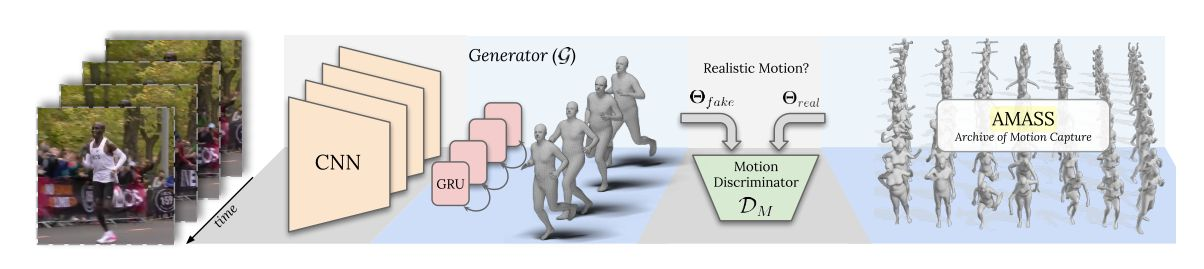
\includegraphics[width=0.5\textwidth]{images/vibe.png}
        \caption{VIBE estimates SMPL parameters from a frame sequence using a temporal encoder trained alongside with a discriminator. The discriminator has access to a large corpus of human motions in SMPL format.}
        \label{vibe_fig}
        \vspace{-4mm}
\end{figure}
The motion discriminator is trained to minimizes the objective function \ref{obj}. Inputs parameters sampled from AMASS dataset $P_R$ are labeled as real, and data generated by the temporal encoder is labeld as fake input.
\begin{equation}
    \label{obj}
    L_{D_M} = E_{\Theta \sim P_{R}}[(D_M(\Theta) - 1)^2] + E_{\Theta \sim P_G}[(D_M(\hat{\Theta}))^2]
\end{equation}
The adversarial loss function for the Encoder is calculated by equation \ref{adv_loss}.
\begin{equation}
L_{adv} = E_{\Theta \sim P_G}[(D_M(\hat{\Theta}) - 1)^2]
\label{adv_loss}
\end{equation}
This loss ensures that parameters estimated by the Temporal encoder belong to the manifold of plausible human motion.
We compare our results with the state-of-the-art methods and outperform all of them in considered datasets. Comparison of the results with some of SOTA methods is shown in Table \ref{tab:my_label}.
\begin{table}[h]
    \centering
    \begin{tabular}{c|c|c}
    \toprule
        & 3DPW & H36M\\
        \midrule
         Kanazawa \bmvaEtAl \cite{kanazawa2018end}& 76.7 & 56.8\\ 
         Doersch \bmvaEtAl \cite{doersch2019sim2real}& 74.7 & -\\
         Sun \bmvaEtAl \cite{sun2019human}& 69.5 & 42.4\\
         VIBE& \textbf{51.9} & \textbf{41.4}\\
         \bottomrule
    \end{tabular}
    \vspace{+3mm}
    \caption{Comparison of VIBE and SOTA methods on 3DPW and H36M datasets reported by Procrustes-aligned mean per joint position error.}
    \label{tab:my_label}
\end{table}

In this paper we discuss VIBE in better details and give implementation technicalities. We also learn a new motion prior from AMASS and show it also helps training but is less powerful than the discriminator. In addition, we perform ablation experiments to examine the enhancement achieved by each part of our proposed model. 
\bibliography{egbib}

\end{document}
